\section{算法的扰动分析}
\label{sec:opt-sto-perturbation}

前面各节分别遇到了几种与理想梯度的偏离：零均值的噪声、裁剪造成的偏差、近似求解的子问题。本节把它们放在一起，问一个共同的问题：固定一个运行有限步的算法，改变它的输入，输出会变多少。输入的改变有两种。一种是方向读数被扰动，数据不变；另一种是数据集中换掉一个样本，算法规则不变。研究对象是“算法映射”，即从数据和随机下标路径到返回点的映射，这与第~\ref{chap:opt-smooth}章研究问题参数变化时\emph{精确}最优解如何移动的敏感性分析不同：那里不涉及算法跑了几步，这里不涉及精确解。

\subsection{读数误差与原目标进展}
\label{sec:opt-sto-reading-error}

\paragraph{三种误差进入递推的位置}
在同一个数据集上，实际方向与真梯度的差可以分成三类。条件噪声$\bm\xi^{(t)}$满足$\mathbb E_t\bm\xi^{(t)}=\bm0$，来自随机抽样。系统偏差$\bm\beta^{(t)}$由历史决定，来自裁剪、量化、过时的参数或有偏的抽样。子问题误差来自块更新、邻近映射或交替最小化中没有精确求解的子问题，若以返回点与精确子问题解的差来计，它也是一个由当前状态决定的偏差。第~\ref{chap:opt-smooth}章已经用这种拆分分析过不精确梯度的梯度下降；这里只把条件期望加进去。

把$\bm g^{(t)}=\nabla f(\bm x^{(t)})+\bm\beta^{(t)}+\bm\xi^{(t)}$代入下降引理，取$\mathbb E_t$。设$\lVert\bm\beta^{(t)}\rVert_2\leq B$，$\mathbb E_t\lVert\bm\xi^{(t)}\rVert_2^2\leq\sigma^2$，$\eta\leq1/L$。记$\bm a=\nabla f(\bm x^{(t)})$，由$-\eta\langle\bm a,\bm a+\bm\beta\rangle+\tfrac\eta2\lVert\bm a+\bm\beta\rVert_2^2=\tfrac\eta2(\lVert\bm\beta\rVert_2^2-\lVert\bm a\rVert_2^2)$，得到
\begin{equation}
\label{eq:opt-sto-biased-step}
  \mathbb E_tf(\bm x^{(t+1)})\leq f(\bm x^{(t)})-\frac\eta2\lVert\nabla f(\bm x^{(t)})\rVert_2^2+\frac\eta2B^2+\frac{L\eta^2}2\sigma^2 .
\end{equation}
求和后与定理~\ref{thm:opt-sto-nonconvex}相同地处理，常数步长下
\[
  \frac1T\sum_{t<T}\mathbb E\lVert\nabla f(\bm x^{(t)})\rVert_2^2\leq\frac{2\bigl(f(\bm x^{(0)})-f_{\inf}\bigr)}{\eta T}+B^2+L\eta\sigma^2 .
\]
三项分别对应初始误差、偏差和噪声。初始误差项随$T$消失；噪声项正比于$\eta$，用小批量还会变成$L\eta\sigma^2/b$；偏差项$B^2$既不依赖$\eta$，也不依赖$T$和批量，是一个硬性的下限。

\paragraph{二次目标上的轨迹}
在二次目标$f(\bm x)=\tfrac12(\bm x-\bm x^\star)^\top\bm H(\bm x-\bm x^\star)$上，轨迹的差可以精确写出：
\[
  \bm x^{(t+1)}-\bm x^\star=(\bm I-\eta\bm H)(\bm x^{(t)}-\bm x^\star)-\eta\bm\beta-\eta\bm\xi^{(t)} .
\]
若偏差是常向量$\bm\beta$，期望迭代收敛到$\bm x^\star-\bm H^{-1}\bm\beta$：偏差把整条轨迹平移到一个新的不动点，平移量$\bm H^{-1}\bm\beta$与步长无关，并在小曲率方向被放大。噪声则在这个点附近造成与$\eta$成正比的波动。图~\ref{fig:opt-sto-perturbation}(a)在二维最小二乘上验证这一点：只有噪声时，误差平台随步长缩小为四分之一而缩小到约四分之一，用$4$个样本的批量效果相同；只有偏差时，两种步长最终停在同一个高度$\lVert\bm H^{-1}\bm\beta\rVert_2^2\approx0.023$，小步长只是到达得更慢。

\begin{figure*}[!htbp]
  \centering
  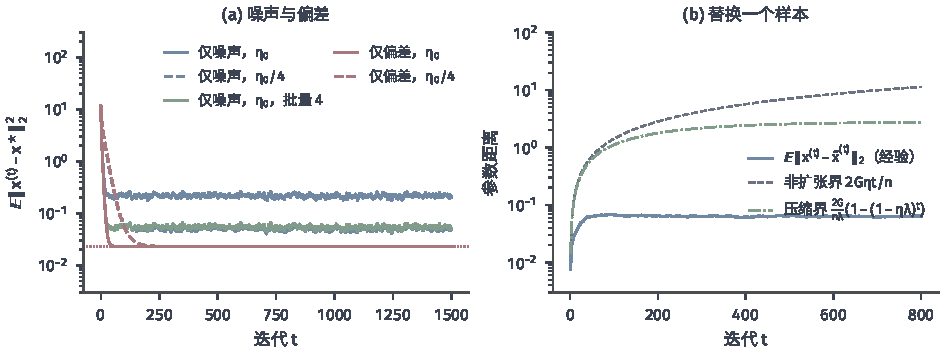
\includegraphics[width=160mm]{figures/03-optimization-evolution-and-signals/01-optimization/matplotlib/c6-perturbation/figure.pdf}
  \caption{两种输入扰动下的算法输出。问题同图~\ref{fig:opt-sto-noise-ball}。(a) 读数为$\nabla f(\bm x)+\bm\beta+\bm\xi/\sqrt b$：仅噪声时$\bm\beta=\bm0$、$\bm\xi\sim N(\bm0,0.25\bm I)$，仅偏差时$\bm\beta=(0.25,0)$、$\bm\xi=\bm0$；$\eta_0=0.4$，$300$次运行平均。红色点线为$\lVert\bm H^{-1}\bm\beta\rVert_2^2$。(b) 把第$1$个样本换成新样本后，以相同初值$\bm0$、相同下标路径和步长$1/L_{\max}$运行两份数据，$2000$次运行的平均参数距离（蓝），以及定理~\ref{thm:opt-sto-stability}的非扩张界与利用正则项强凸性的压缩界，纵轴为对数坐标。$G\approx2.78$是两条路径上被替换两项梯度范数的最大值。}
  \label{fig:opt-sto-perturbation}
\end{figure*}

\paragraph{哪种手段改善哪一项}
这个分解说明了常见调节手段各自作用于哪一项。增大批量或缩小步长只压低噪声项。去掉偏差需要改变读数本身：放宽裁剪阈值、使用无偏的抽样权重、使用更新的参数。子问题误差则要靠把子问题解得更准来减小，每一轮的子问题误差都像偏差一样进入递推。如果偏差项已经占主导，继续增大批量或延长运行都无济于事。

\paragraph{带历史的方法与不同的误差对象}
动量、Adam、SAGA这类方法的下一步不仅取决于当前参数，还取决于动量、统计量或梯度表。比较两次运行时，必须把完整状态作为比较对象：参数相同而动量不同，未来的轨迹也不同。另外要区分三种误差对象：目标误差邻域（期望目标差停在多高）、期望驻点残差（梯度范数平方的平均）以及实际轨迹的偏差（某次运行与参考轨迹的距离）。随机梯度运行中目标估计值的波动，很大部分来自评估目标所用的抽样，不直接等于参数不稳定；反过来，参数几乎不动也不说明已经接近最优，偏差项可能正把它固定在一个错误的位置。

\subsection{样本替换的有限步响应}
\label{sec:opt-sto-stability}

\paragraph{耦合两次运行}
现在固定读数规则，改变数据。设数据集$S$与$S'$只有第$k$个样本不同，对应的逐项函数为$f_i$与$f_i'$，$i\neq k$时$f_i=f_i'$。在两份数据上运行随机梯度下降，使用相同的初值、相同的步长和\emph{相同的}下标序列$i^{(0)},i^{(1)},\dots$，得到$\bm x^{(t)}$与$\tilde{\bm x}^{(t)}$。这种耦合把抽样噪声的影响去掉，两条轨迹的差只来自被替换的样本。

\paragraph{非扩张的梯度步}
没有抽到第$k$项时，两条轨迹用同一个函数$f_i$走一步。下面的性质说明这一步不会拉开距离。

\begin{lemma}[凸光滑函数梯度步的非扩张性]
\label{lem:opt-sto-nonexpansive}
设$\phi$凸且$L$光滑，$0\leq\eta\leq2/L$。则对任意$\bm x,\bm y$，$\lVert(\bm x-\eta\nabla\phi(\bm x))-(\bm y-\eta\nabla\phi(\bm y))\rVert_2\leq\lVert\bm x-\bm y\rVert_2$。
\end{lemma}

\begin{proof}
把引理~\ref{lem:opt-sto-cocoercive}分别用于$(\bm x,\bm y)$和$(\bm y,\bm x)$再相加，函数值项相消，得到$\lVert\bm\Delta\rVert_2^2\leq L\langle\bm\Delta,\bm x-\bm y\rangle$，其中$\bm\Delta=\nabla\phi(\bm x)-\nabla\phi(\bm y)$。于是
$\lVert\bm x-\bm y-\eta\bm\Delta\rVert_2^2=\lVert\bm x-\bm y\rVert_2^2-2\eta\langle\bm\Delta,\bm x-\bm y\rangle+\eta^2\lVert\bm\Delta\rVert_2^2\leq\lVert\bm x-\bm y\rVert_2^2-\eta(2/L-\eta)\lVert\bm\Delta\rVert_2^2$，当$\eta\leq2/L$时最后一项非正。
\end{proof}

\begin{theorem}[样本替换下的期望参数距离]
\label{thm:opt-sto-stability}
设每个$f_i$与$f_k'$凸且$L$光滑，下标独立均匀抽取，确定的步长满足$0\leq\eta^{(t)}\leq2/L$，并设在两条轨迹访问过的点上，被替换的两项梯度满足$\lVert\nabla f_k(\bm x^{(t)})\rVert_2\leq G$与$\lVert\nabla f_k'(\tilde{\bm x}^{(t)})\rVert_2\leq G$。则
\begin{equation}
\label{eq:opt-sto-stability}
  \mathbb E\lVert\bm x^{(T)}-\tilde{\bm x}^{(T)}\rVert_2\leq\frac{2G}{n}\sum_{t<T}\eta^{(t)} .
\end{equation}
\end{theorem}

\begin{proof}
记$\delta_t=\lVert\bm x^{(t)}-\tilde{\bm x}^{(t)}\rVert_2$，$\delta_0=0$。若$i^{(t)}\neq k$，两条轨迹对同一个$f_i$作梯度步，由引理~\ref{lem:opt-sto-nonexpansive}，$\delta_{t+1}\leq\delta_t$。若$i^{(t)}=k$，由三角不等式，$\delta_{t+1}\leq\delta_t+\eta^{(t)}\bigl(\lVert\nabla f_k(\bm x^{(t)})\rVert_2+\lVert\nabla f_k'(\tilde{\bm x}^{(t)})\rVert_2\bigr)\leq\delta_t+2\eta^{(t)}G$。下标与历史独立，后一种情形的条件概率为$1/n$，所以$\mathbb E_t\delta_{t+1}\leq\delta_t+2\eta^{(t)}G/n$。取全期望并累加即得。
\end{proof}

这个界的结构很直观：每一步以概率$1/n$注入至多$2\eta^{(t)}G$的差异，注入之后的差异不会被后续步骤放大。若每项还是$\lambda$强凸的且二阶连续可微，$\eta\leq2/(L+\lambda)$时梯度步的Jacobian$\bm I-\eta\nabla^2f_i$的特征值落在$[-(1-\eta\lambda),1-\eta\lambda]$内，非扩张可以加强为以因子$1-\eta\lambda$压缩，差异的递推变为$\mathbb E\delta_{t+1}\leq(1-\eta\lambda)\mathbb E\delta_t+2\eta G/n$，界不再随$T$无限增长，而是停在$2G/(n\lambda)$以下。图~\ref{fig:opt-sto-perturbation}(b)中，平均距离在约$50$步内升到约$0.06$后保持稳定；非扩张界随$t$线性增长，在$t=20$时已是实际值的约$7$倍，压缩界则趋于约$2.7$。两个界都正确但偏保守，原因是$G$取了路径上的最大值，而实际注入的差异多数时候远小于$2\eta G$。

\paragraph{这个界说明了什么，没有说明什么}
式~\eqref{eq:opt-sto-stability}描述的是运行有限步的算法映射对单个样本的敏感程度，属于\term{算法稳定性}（algorithmic stability）的一种形式\scite{hardt2016sgd}。它与固定目标下的抽样噪声是两回事：同一份数据、不同下标路径的两次运行，距离由噪声邻域决定，可能比这里的距离大得多；这里刻意用同一条下标路径把那部分去掉。条件也需要逐项核对：要求的是\emph{每一项}凸，而不只是平均目标凸；梯度界$G$只需在实际访问的点上对被替换的两项成立，对最小二乘这样梯度随参数增长的目标，它依赖于轨迹停留的区域。若要把参数距离转为损失之差，还需要损失对参数的Lipschitz常数$K$，得到$|\ell(\bm x^{(T)};z)-\ell(\tilde{\bm x}^{(T)};z)|\leq K\lVert\bm x^{(T)}-\tilde{\bm x}^{(T)}\rVert_2$。至于从这里推出关于未见数据的泛化结论，还需要统计论证，由后续讨论学习理论的部分承担。
